\subsection{Problem 5}%
\label{sec:problem_5}
A missile is fired from enemy territory, and its position in flight is observed by radar
tracking devices at the following positions:
\begin{center}
  \begin{tabular}{|c|c|c|c|c|c|}
    \hline
    $x_i$ [km] & 0 & 250 & 500 & 750 & 1000 \\
    \hline
    $y_i$ [km] & 0 & 8 & 15 & 19 & 20 \\
    \hline
  \end{tabular}
\end{center}
Suppose our intelligence sources indicate that enemy missiles are programmed to follow a
parabolic flight path. Predict how far down range the missile will land.
%%%%%%%%%%%%%%%%%%%%%%%%%%%%%%%%%%%%%%%%%%%%%%%%%%%%%%%%%%%%%%%%%%%%%%%%%%%%%%%
\subsubsection*{Mathematics}
%%%%%%%%%%%%%%%%%%%%%%%%%%%%%%%%%%%%%%%%%%%%%%%%%%%%%%%%%%%%%%%%%%%%%%%%%%%%%%%
This problem may be solved with the linear regression approach just like the previous
one.
The only difference is the degree of polynomial which we want to fit into the data
points --- in the case of the parabolic flight it is a quadratic function.
Once it is found, predicting the range of the missile is finding the second root.
%%%%%%%%%%%%%%%%%%%%%%%%%%%%%%%%%%%%%%%%%%%%%%%%%%%%%%%%%%%%%%%%%%%%%%%%%%%%%%%
\subsubsection*{Solution}
%%%%%%%%%%%%%%%%%%%%%%%%%%%%%%%%%%%%%%%%%%%%%%%%%%%%%%%%%%%%%%%%%%%%%%%%%%%%%%%
Once again we may use the normal equations to approximate the solution to the equation
$y = a_0 + a_1x + a_2x^2$.
Following the suggestion from~\cite{Meyer}, we scale the $x$ to the kkm:
\lstinputlisting[style=Matlab-editor]{problems/Problem_5.m}
from which we conclude that the missile, whose trajectory may be seen in
the~\autoref{fig:problem_5}, will land at the range of 2044.2 km.
\begin{figure}
  \centering
  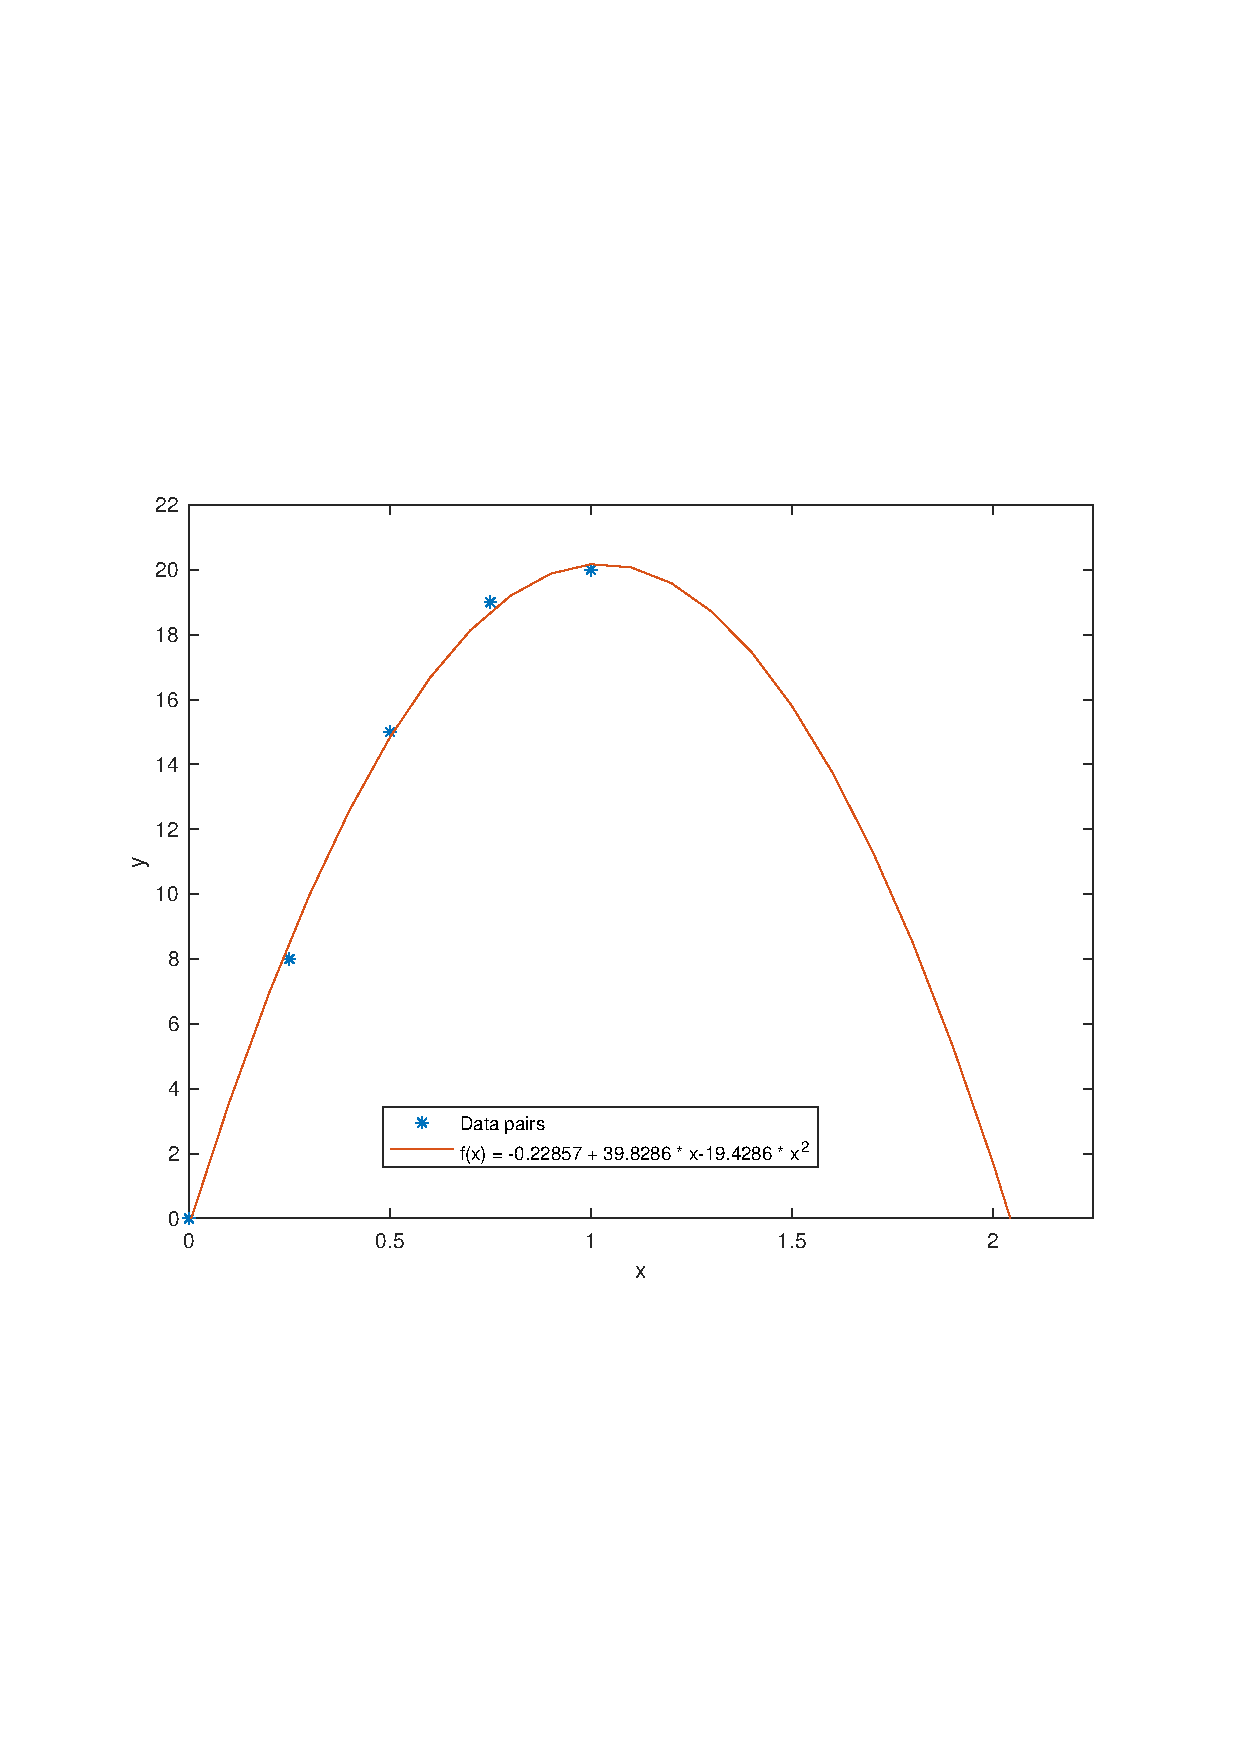
\includegraphics[width=0.7\textwidth]{images/Problem_5_plot.pdf}
  \caption{The plot of the approximated missile trajectory and the provided data points}
  \label{fig:problem_5}
\end{figure}
